\documentclass[10pt]{beamer}

\usetheme{metropolis}

\usepackage[export]{adjustbox}
\usepackage{hyperref}
\usepackage{listings}
\usepackage{pgfplots}
\usepackage{tikz}
\usepackage{xcolor}

\usepgfplotslibrary{fillbetween}

\usetikzlibrary{arrows}
\usetikzlibrary{arrows.meta}
\usetikzlibrary{calc}
\usetikzlibrary{fadings}
\usetikzlibrary{patterns}
\usetikzlibrary{positioning}

\hypersetup{
    colorlinks=true,
    linkcolor=white,
    urlcolor=blue!80
}

\definecolor{uiored}{HTML}{DD0000}
\definecolor{uiolightred}{HTML}{FB6666}
\definecolor{uioredtone}{HTML}{FEE0E0}
\definecolor{uioblue}{HTML}{3E31D6}
\definecolor{uiolightblue}{HTML}{86A4F7}
\definecolor{uioblueone}{HTML}{E6ECFF}
\definecolor{uiogreen}{HTML}{2EC483}
\definecolor{uiolightgreen}{HTML}{6CE1AB}
\definecolor{uiogreentone}{HTML}{CEFFDF}
\definecolor{uioorange}{HTML}{FEA11B}
\definecolor{uiolightorange}{HTML}{FDCB87}
\definecolor{uioorangetone}{HTML}{FFE8D4}
\definecolor{uioyellow}{HTML}{FFFEA7}
\definecolor{uiogray}{HTML}{B2B3B7}

\colorlet{mainbackground}{uiored}

\setbeamercolor{frametitle}{bg=mainbackground, fg=white}
\setbeamercolor{title separator}{fg=mainbackground}
\setbeamercolor{progress bar in section page}{fg=white, bg=uiogray}

\def\logowidth{4cm}

\makeatletter
\setbeamertemplate{section page}
{
  \begingroup

    \vspace{4.3cm}
    {\usebeamercolor[fg]{section title}\usebeamerfont{section title}\insertsectionhead}\\[-1ex]
    {\centering\color{white}\rule{\linewidth}{1pt}\par} % the horizontal line

    \vspace*{3.1cm}
    \begin{center}
        
\includegraphics[width=\logowidth,valign=c]{data/uio_logo_full_white.png} % Adjust width and path to your logo as needed
    \end{center}

  \endgroup
}
\makeatother

\AtBeginSection{
  {
    \setbeamercolor{background canvas}{bg=uiored}
    \setbeamercolor{section title}{fg=white}
    \frame[plain,c,noframenumbering]{\sectionpage}
    \setbeamercolor{background canvas}{bg=black!2}
  }
}



\setbeamertemplate{footline}{
    \ifnum\insertframenumber=1
        % Title page, no footer
    \else
        \begin{tikzpicture}[remember picture,overlay]
            \fill[mainbackground] (current page.south west) rectangle ([yshift=0.45cm]current page.south east); % Draw filled rectangle

            % Logo
            \node[anchor=west, yshift=0.225cm] at (current page.south west) {
\includegraphics[height=1.2cm]{data/uio_logo_white.png}};

            % Title and subtitle
            \node[align=center, yshift=0.225cm] at (current page.south) {\textcolor{white}{\textbf{\inserttitle}}\\[0.05cm]\textcolor{white}{\insertsubtitle}};

            % Page number
            \node[anchor=east, yshift=0.225cm, xshift=-0.2cm, align=right] at (current page.south east) {\textcolor{white}{\insertframenumber/\inserttotalframenumber}};
        \end{tikzpicture}
    \fi
}

\newcommand{\stickman}[2]{
    \node[circle,fill,minimum size=5mm,#2] (head) at #1 {};
    \node[rounded corners=1pt,minimum height=1.3cm,minimum width=0.4cm,fill,below = 0.5pt of head,#2] (body) {};
    \draw[line width=1mm,round cap-round cap,#2] ([shift={(2pt,-0.5pt)}]body.north east) --++(-90:6mm);
    \draw[line width=1mm,round cap-round cap,#2] ([shift={(-2pt,-0.5pt)}]body.north west)--++(-90:6mm);
    \draw[thick,white,-round cap] (body.south) --++(90:5.5mm);
}

\newcommand{\stickmantorso}[2]{
    \node[circle,fill,minimum size=5mm,#2] (head) at #1 {};
    \node[rounded corners=1pt,minimum height=0.8cm,minimum width=0.15cm,fill,below left= 0.6cm + 0.5pt and -0.145cm of head,draw=#2, fill=white, inner sep=0pt] (leftleg) {};
    \node[rounded corners=1pt,minimum height=0.8cm,minimum width=0.15cm,fill,below right= 0.6cm + 0.5pt and -0.145cm of head,draw=#2, fill=white, inner sep=0pt] (rightleg) {};
    \node[rounded corners=1pt,minimum height=0.6cm,minimum width=0.4cm,fill,below = 0.5pt of head,#2] (torso) {};
    \node[minimum height=0.6cm,minimum width=0.4cm,fill,below = 0.1cm + 0.5pt of head,#2] {};
    \draw[line width=1mm,round cap-round cap,#2] ([shift={(2pt,-0.5pt)}]torso.north east) --++(-90:6mm);
    \draw[line width=1mm,round cap-round cap,#2] ([shift={(-2pt,-0.5pt)}]torso.north west)--++(-90:6mm);
}

\newcommand{\stickmanlegs}[2]{
    \node[circle,fill,minimum size=5mm,draw=#2,fill=white] (head) at #1 {};
    \node[rounded corners=1pt,minimum height=0.8cm,minimum width=0.16cm,fill,below left= 0.6cm + 0.5pt and -0.145cm of head,#2, inner sep=0pt] (leftleg) {};
    \node[rounded corners=1pt,minimum height=0.8cm,minimum width=0.16cm,fill,below right= 0.6cm + 0.5pt and -0.145cm of head,#2, inner sep=0pt] (rightleg) {};
    \node[rounded corners=1pt,minimum height=0.7cm,minimum width=0.4cm,fill,below = 0.5pt of head,fill=white, draw=#2] (torso) {};
    \draw[rounded corners=1pt, draw=#2, fill=white, line width=0.1mm] ([shift={(1pt,-0.5pt)}]torso.north east) --++(-90:6mm) --++(1mm,0) --++(0,6mm) --++(-1mm,0);
    \draw[rounded corners=1pt, draw=#2, fill=white, line width=0.1mm] ([shift={(-1pt,-0.5pt)}]torso.north west) --++(-90:6mm) --++(-1mm,0) --++(0,6mm) --++(1mm,0);
}

\newcommand{\stickmanleft}[2]{
    \node[circle,fill,minimum size=5mm,draw=#2,fill=white] (head) at #1 {};
    \node[rounded corners=1pt,minimum height=0.8cm,minimum width=0.16cm,fill,below left= 0.6cm + 0.5pt and -0.145cm of head,draw=#2, fill=white, inner sep=0pt] (leftleg) {};
    \node[rounded corners=1pt,minimum height=0.8cm,minimum width=0.16cm,fill,below right= 0.6cm + 0.5pt and -0.145cm of head,#2, inner sep=0pt] (rightleg) {};
    \node[rounded corners=1pt,minimum height=0.7cm,minimum width=0.4cm,fill,below = 0.5pt of head,fill=white, draw=#2] (torso) {};
    \draw[rounded corners=1pt, draw=#2, fill=white, line width=0.1mm] ([shift={(1pt,-0.5pt)}]torso.north east) --++(-90:6mm) --++(1mm,0) --++(0,6mm) --++(-1mm,0);
    \draw[rounded corners=1pt, draw=#2, fill=white, line width=0.1mm] ([shift={(-1pt,-0.5pt)}]torso.north west) --++(-90:6mm) --++(-1mm,0) --++(0,6mm) --++(1mm,0);
}

\newcommand{\stickmanright}[2]{
    \node[circle,fill,minimum size=5mm,draw=#2,fill=white] (head) at #1 {};
    \node[rounded corners=1pt,minimum height=0.8cm,minimum width=0.16cm,fill,below left= 0.6cm + 0.5pt and -0.145cm of head,#2, inner sep=0pt] (leftleg) {};
    \node[rounded corners=1pt,minimum height=0.8cm,minimum width=0.16cm,fill,below right= 0.6cm + 0.5pt and -0.145cm of head, draw=#2, fill=white, inner sep=0pt] (rightleg) {};
    \node[rounded corners=1pt,minimum height=0.7cm,minimum width=0.4cm,fill,below = 0.5pt of head,fill=white, draw=#2] (torso) {};
    \draw[rounded corners=1pt, draw=#2, fill=white, line width=0.1mm] ([shift={(1pt,-0.5pt)}]torso.north east) --++(-90:6mm) --++(1mm,0) --++(0,6mm) --++(-1mm,0);
    \draw[rounded corners=1pt, draw=#2, fill=white, line width=0.1mm] ([shift={(-1pt,-0.5pt)}]torso.north west) --++(-90:6mm) --++(-1mm,0) --++(0,6mm) --++(1mm,0);
}

\title{Entrepeneurship}
\subtitle{A viable option after/during a PhD?}
\author{Esten H. Leonardsen}
\date{06.06.24}

\titlegraphic{
	\centering
	\vspace{7.7cm}
	
\includegraphics[width=\logowidth]{data/uio_logo_full.png}
}

\definecolor{firstcolor}{HTML}{ef476f}
\definecolor{secondcolor}{HTML}{ffd166}
\definecolor{thirdcolor}{HTML}{06d6a0}
\definecolor{fourthcolor}{HTML}{118ab2}
\definecolor{snapsalecolor}{HTML}{ff0058}
\definecolor{epigramcolor}{HTML}{59d38a}
\definecolor{medtechcolor}{HTML}{4a4a4a}
\definecolor{biocolor}{HTML}{0aaeed}
\definecolor{sportaicolor}{HTML}{02583f}
\definecolor{babacolor}{HTML}{3ae5be}
\definecolor{plasticcolor}{HTML}{235877}

\begin{document}
	\begin{frame}
	 	\titlepage
	\end{frame}

    \begin{frame}{Overview}
        \begin{enumerate}
            \item How is life in a start-up?
            \item Things to keep in mind
            \item Useful resources
        \end{enumerate}
    \end{frame}

    \section{Why should you listen to me?}

    \begin{frame}{Background}
        \centering
        \begin{tikzpicture}
            \node[] at (0, 0) {
                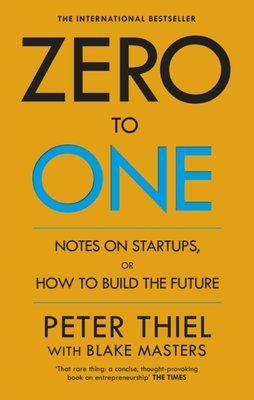
\includegraphics[height=4.5cm]{data/thiel.jpeg}
            };
            \node[] at (3.75, 0) {
                
\includegraphics[height=4.5cm]{data/lean.jpeg}
            };
            \node[] at (7.5, 0) {
                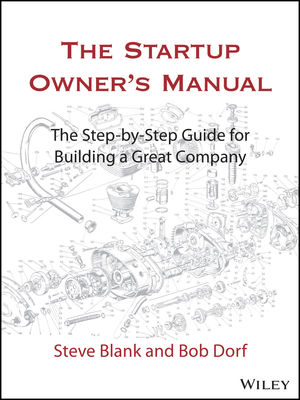
\includegraphics[height=4.5cm]{data/manual.jpeg}
            };
        \end{tikzpicture}
    \end{frame}

    \begin{frame}{Background}
        \centering
        \begin{tikzpicture}
            \node[] at (0, 0) {};
            \node[] at (11, -7) {};

            \only<1-3,6-7,9-21>{
                \draw[-stealth] (0.5, -6) -- (9.5, -6);
                \node[anchor=north] (2016) at (1, -6) {2016};
                \node[anchor=north] (2017) at (2, -6) {2017};
                \node[anchor=north] (2018) at (3, -6) {2018};
                \node[anchor=north] (2019) at (4, -6) {2019};
                \node[anchor=north] (2020) at (5, -6) {2020};
                \node[anchor=north] (2021) at (6, -6) {2021};
                \node[anchor=north] (2022) at (7, -6) {2022};
                \node[anchor=north] (2023) at (8, -6) {2023};
                \node[anchor=north] (2024) at (9, -6) {2024};

                \foreach \year in {2016,...,2024} {
                    \draw[] ($ (\year.north) - (0, 0.05) $) -- ($ (\year.north) + (0, 0.05) $);
                }

                \def\descriptionsize{\footnotesize}

                \draw[uiored, line width=2pt] ($ (2020.north) + (0, 5.5) $) -- ($ (2024.north) + (0, 5.5) $);
                \node[] at ($ (2020.north) + (0, 5.5) $) {
                    
\includegraphics[width=0.5cm]{data/uio_logo.png}
                };
                \only<1> {
                    \node[anchor=south, inner sep=0pt, font=\descriptionsize] at ($ (2022.north) + (0, 5.55) $) {PhD Psychology};
                }

                \pgfdeclarehorizontalshading{blacktored}{100bp}{
                    color(0bp)=(black);
                    color(100bp)=(red)
                }
                \onslide<2->{
                    \node[
                        inner sep=0pt,
                        minimum height=2pt,
                        fill=black,
                        minimum width=1cm,
                        left color=black!2,
                        right color=uiored,
                        draw=none
                    ] at ($ (2016.north) + (-0.5, 5) $) {};
                }
                \only<2>{
                    \node[font=\descriptionsize, align=left, anchor=west] at ($ (2016.north) + (0, 5) $) {
                        MSc. Computer Science
                    };
                }
                \onslide<3->{
                    \onslide<6->{
                        \draw[snapsalecolor, line width=2pt] ($ (2016.north) + (-0.1, 4.5) $) -- ($ (2017.north) + (0, 4.5) $);
                    }
                    \node[anchor=east, inner sep=0pt] (snapsale) at ($ (2016.north) + (0, 4.5) $) {
                        
\includegraphics[width=0.5cm]{data/snapsale.png}
                    };
                    \only<3>{
                        \node[anchor=west, align=left, font=\descriptionsize\linespread{0.8}\selectfont, text depth=0] at (snapsale.east) {
                            \textbf{Snapsale}\\
                            Developer
                        };
                    }
                }
                \onslide<7->{
                    \onslide<8->{
                        \draw[epigramcolor, line width=2pt] ($ (2017.north) + (0, 4) $) -- ($ (2018.north) + (0, 4) $);
                    }
                    \node[draw=black, inner sep=0pt, fill=white, anchor=east] (epigram) at ($ (2017.north) + (0, 4) $) {
                        
\includegraphics[width=0.5cm]{data/epigram.png}
                    };
                    \only<7>{
                        \node[anchor=west, align=left, font=\descriptionsize\linespread{0.8}\selectfont, text depth=0] at (epigram.east) {
                            \textbf{Epigram}\\
                            Co-founder, board member, lead data scientist
                        };
                    }
                }
                \onslide<9->{
                    \onslide<10->{
                        \draw[medtechcolor, line width=2pt] ($ (2018.north) + (0, 3.5) $) -- ($ (2020.north) + (1, 3.5) $);
                        \draw[medtechcolor!20, line width=2pt] ($ (2020.north) + (0, 3.5) $) -- ($ (2024.north) + (0, 3.5) $);
                        \draw[medtechcolor, line width=2pt,-stealth] ($ (2024.north) + (0, 3.5) $) -- ($ (2024.north) + (1, 3.5) $);
                    }
                    \node[draw=black, inner sep=0pt, fill=white, anchor=east] (medtech) at ($ (2018.north) + (0, 3.5) $) {
                        
\includegraphics[height=0.5cm]{data/medtech.png}
                    };
                    \only<9>{
                        \node[anchor=west, align=left, font=\descriptionsize\linespread{0.8}\selectfont, text depth=0] at (medtech.east) {
                            \textbf{Epigram medtech}\\
                            Founder, chairman of the board, CEO, consultant
                        };
                    }
                }
                \onslide<11->{
                    \onslide<12->{
                        \draw[black, line width=2pt] ($ (2020.north) + (-0.1, 3) $) -- ($ (2021.north) + (0, 3) $);
                    }
                    \node[anchor=east, inner sep=0pt] (solv) at ($ (2020.north) + (0, 3) $) {
                        
\includegraphics[height=0.5cm]{data/solv.png}
                    };
                    \only<11>{
                        \node[anchor=west, align=left, font=\descriptionsize\linespread{0.8}\selectfont, text depth=0] at (solv.east) {
                            \textbf{Solv Oslo}\\
                            Scientific advisor
                        };
                    }
                }
                \onslide<13->{
                    \onslide<14->{
                        \draw[biocolor, line width=2pt,-stealth] ($ (2021.north) + (0, 2.5) $) -- ($ (2024.north) + (1, 2.5) $);
                    }
                    \node[draw=black, inner sep=0pt, fill=white,anchor=east] (bio) at ($ (2021.north) + (0, 2.5) $) {
                        
\includegraphics[height=0.5cm]{data/biometrical.jpeg}
                    };
                    \only<13>{
                        \node[anchor=west, align=left, font=\descriptionsize\linespread{0.8}\selectfont, text depth=0] at (bio.east) {
                            \textbf{Biometrical}\\
                            Founder, chairman of the board
                        };
                    }
                }
                \onslide<15->{
                    \onslide<16->{
                        \draw[sportaicolor, line width=2pt, -stealth] ($ (2024.north) + (-0.1, 2) $) -- ($ (2024.north) + (1, 2) $);
                    }
                    \node[anchor=east, inner sep=0pt] (sportai) at ($ (2024.north) + (0, 2) $) {
                        
\includegraphics[height=0.37cm]{data/sportai.jpeg}
                    };
                    \only<15>{
                        \node[anchor=west, align=left, font=\descriptionsize\linespread{0.8}\selectfont, text depth=0] at (sportai.east) {
                            \textbf{SportAI}\\
                            Advisor
                        };
                    }
                }

                \onslide<17->{
                    \onslide<18->{
                        \draw[plasticcolor, line width=2pt, -stealth] ($ (2024.north) + (0, 1.5) $) -- ($ (2024.north) + (1, 1.5) $);
                    }
                    \node[draw=black, anchor=east, inner sep=0pt] (plastic) at ($ (2024.north) + (0, 1.5) $) {
                        
\includegraphics[height=0.45cm]{data/plastic.jpeg}
                    };
                    \only<17>{
                        \node[anchor=west, align=left, font=\descriptionsize\linespread{0.8}\selectfont, text depth=0] at (plastic.east) {
                            \textbf{Plastic-I}\\
                            Consultant
                        };
                    }
                }

                \onslide<19->{
                    \onslide<20->{
                        \draw[babacolor, line width=2pt, -stealth] ($ (2024.north) + (0, 1) $) -- ($ (2024.north) + (1, 1) $);
                    }
                    \node[draw=black, anchor=east, inner sep=0pt] (baba) at ($ (2024.north) + (0, 1) $) {
                        
\includegraphics[height=0.38cm]{data/baba_logo.png}
                    };
                    \only<19>{
                        \node[anchor=west, align=left, font=\descriptionsize\linespread{0.8}\selectfont, text depth=0] at (baba.east) {
                            \textbf{baba.vision}\\
                            CTO
                        };
                    }
                }
            }
            \only<4>{
                \node[inner sep=0pt, draw=black] at (5, -3.5) {
                    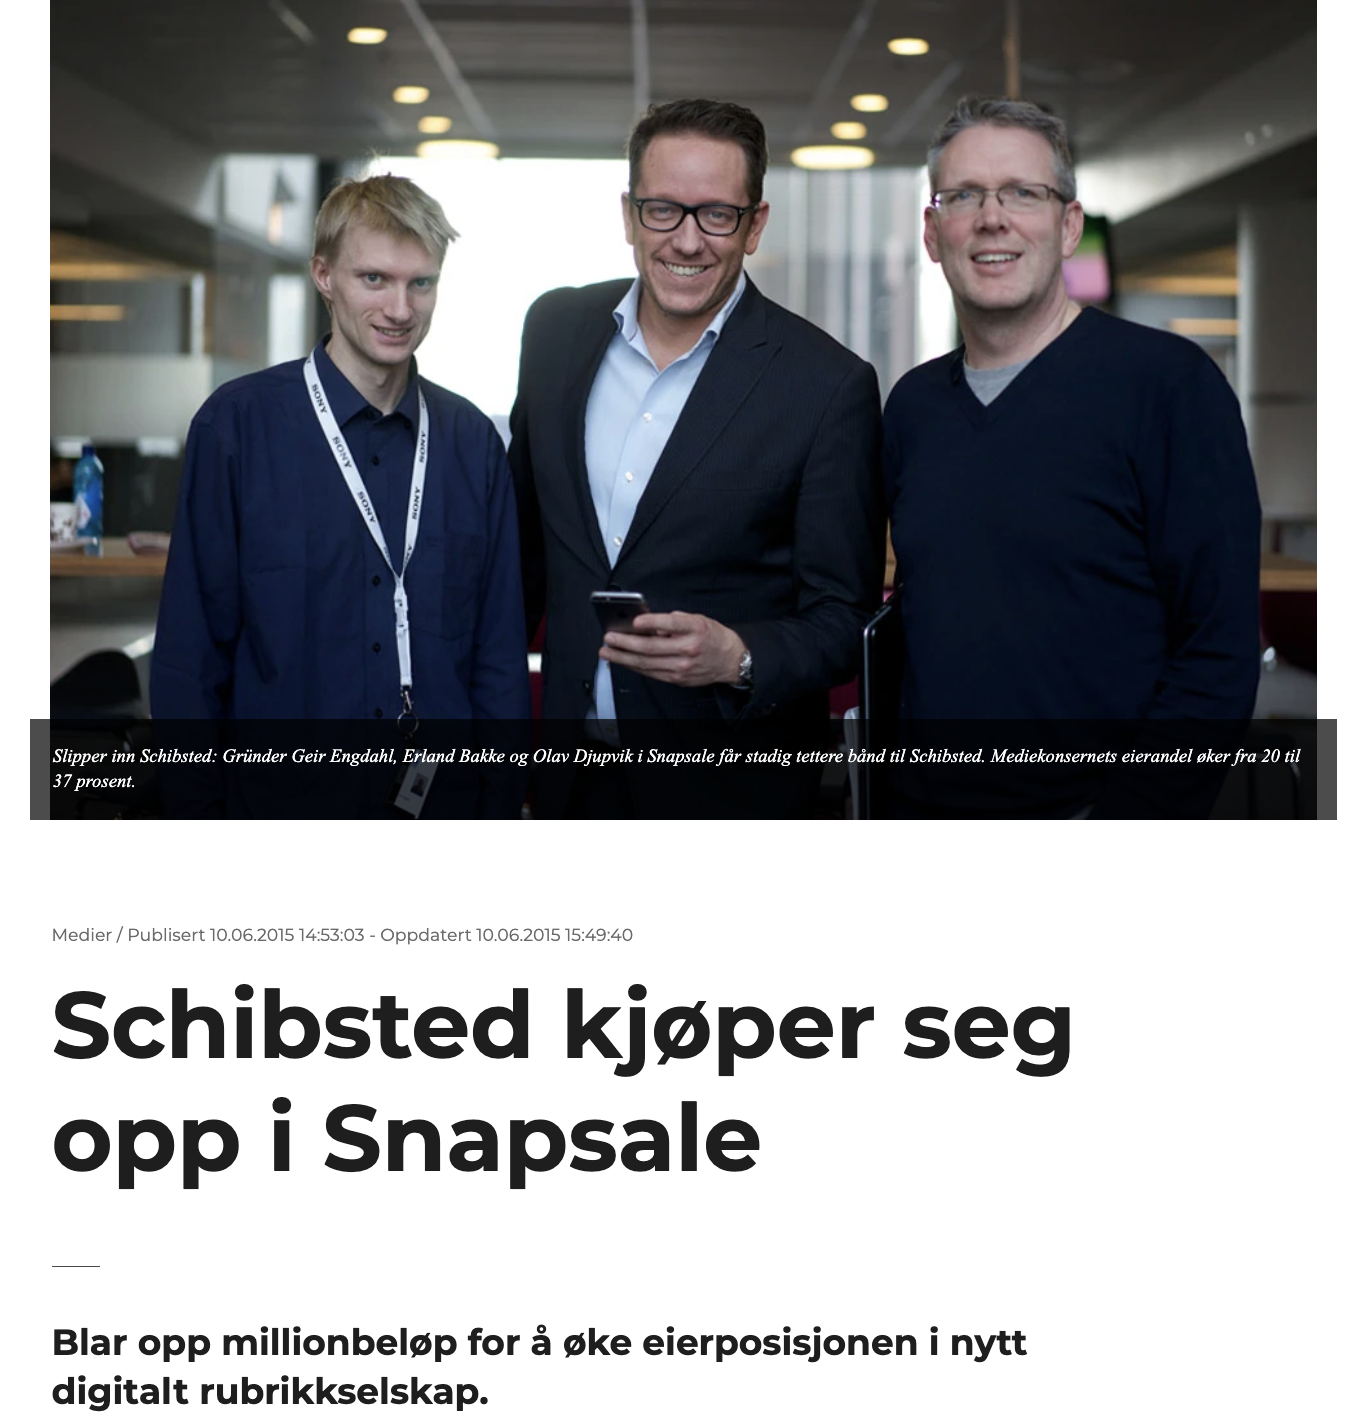
\includegraphics[width=6cm]{data/investering.png}
                };
            }
            \only<5>{
                \node[inner sep=0pt, draw=black] at (5, -3.5) {
                    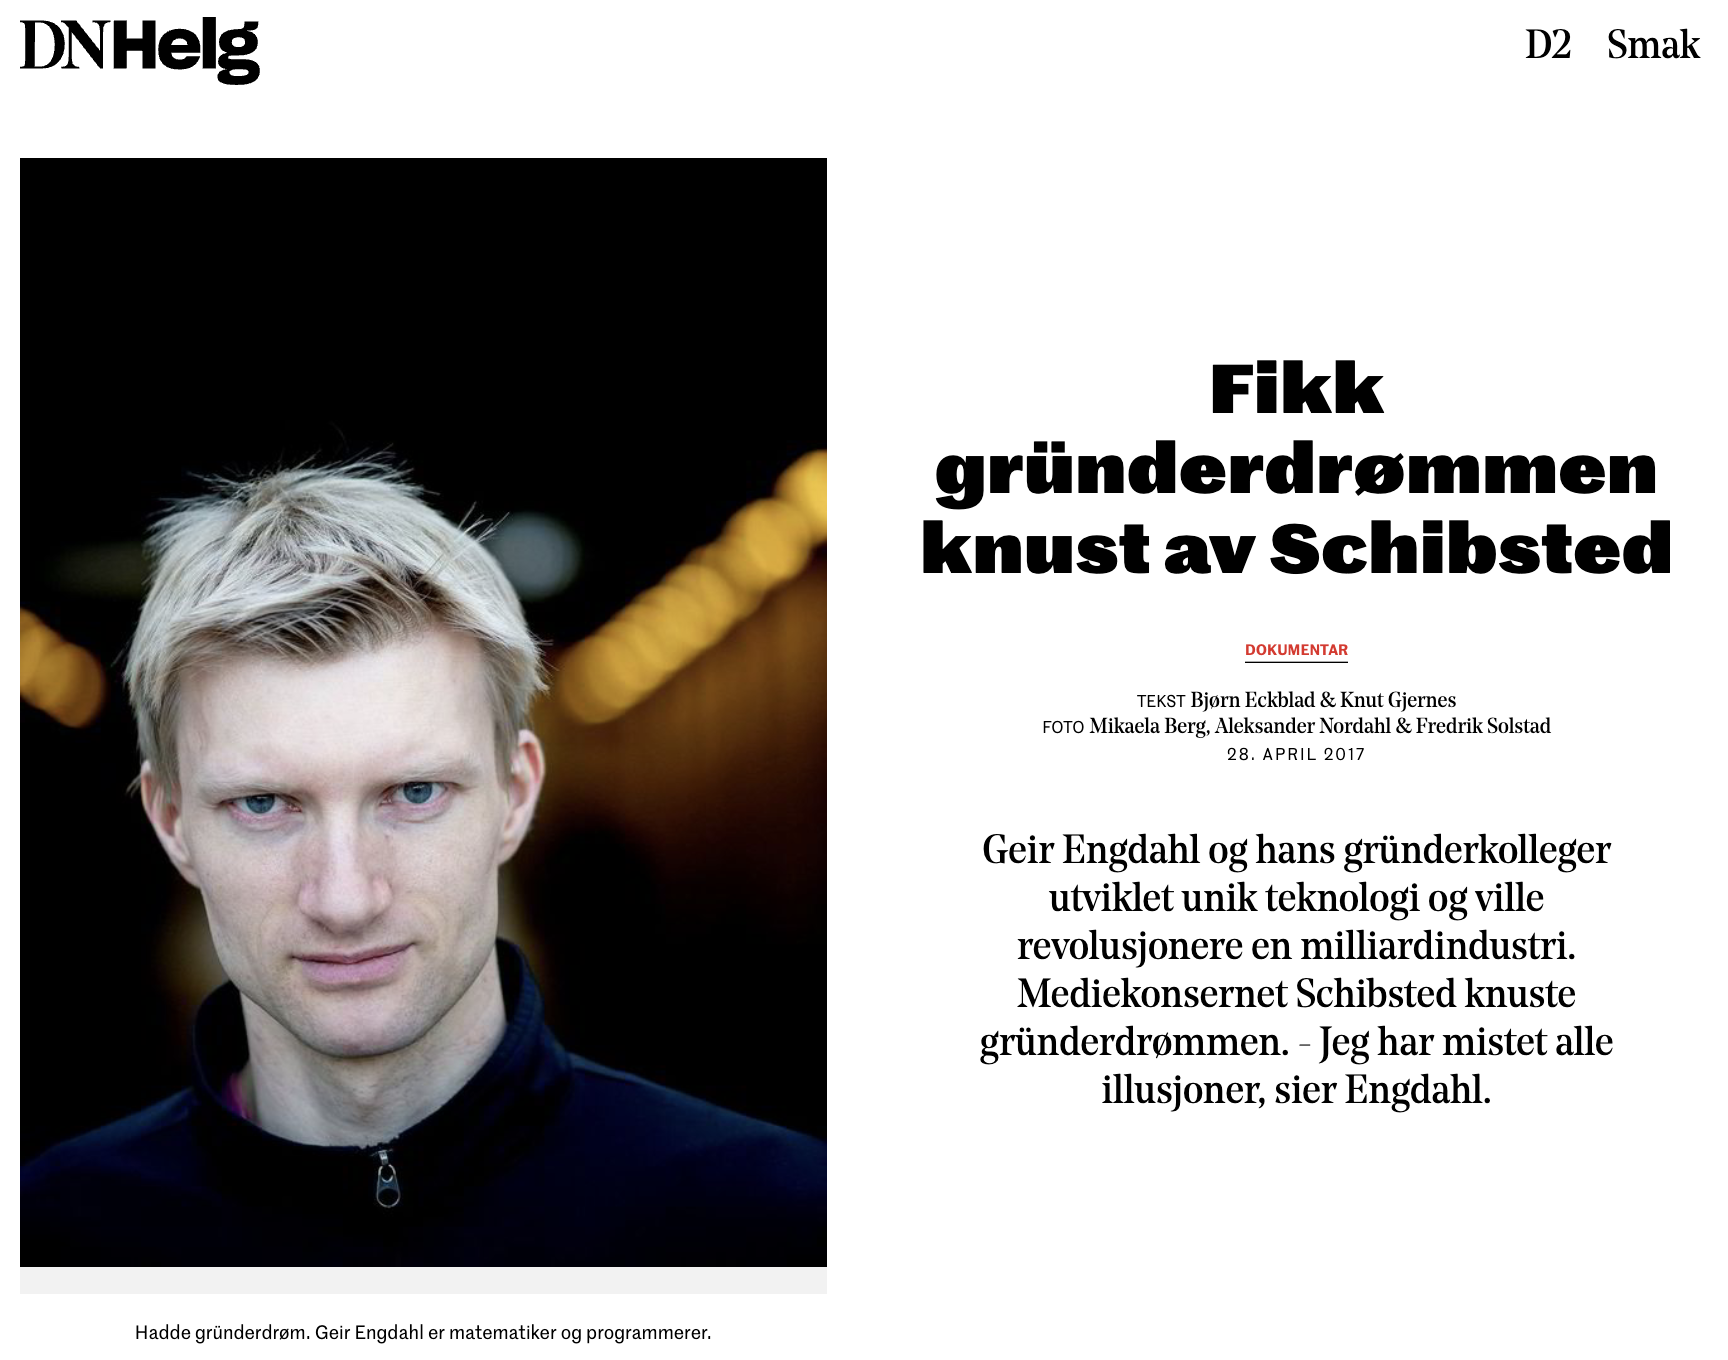
\includegraphics[width=8cm]{data/knust.png}
                };
            }
        \end{tikzpicture}
    \end{frame}

    \section{How is life as an entrepeneur/in a start-up?}

    \begin{frame}{Start-up life}
        \begin{tikzpicture}
            \node[] at (0, 0) {};
            \node[] at (10, -7) {};

            \node[] (happy) at (2, -1.55) {
                
\includegraphics[width=3cm]{data/happy_student.png}
            };
            \only<1-6>{
                \node[anchor=north west, align=left] at (happy.north east) {
                    \begin{minipage}{10cm}
                        \textbf{\underline{Advantages of being a PhD student}}
                        \only<2-6>{
                            \begin{itemize}
                                \item Focus on what matters to you
                                \only<3-6>{\item Freedom}
                                \only<5-6>{\item Room for personal growth}
                                \only<6>{\item Inspiring environment}
                            \end{itemize}
                        }
                    \end{minipage}
                };
            }
            \node[] (sad) at (2, -5.45) {
                
\includegraphics[width=3cm]{data/sad_student.png}
            };
            \only<1-6>{
                \node[anchor=north west, align=left] at (sad.north east) {
                    \begin{minipage}{10cm}
                        \textbf{\underline{Disadvantages of being a PhD student}}
                        \only<3-6>{
                            \begin{itemize}
                                \item Responsibility
                                \only<4-6>{\item Stressful}
                            \end{itemize}
                        }
                    \end{minipage}
                };
            }

            \onslide<7->{
                \node[] at (2, -1.55) {
                    
\includegraphics[width=3cm]{data/happy_suit.png}
                };
                \node[] at (2, -5.45) {
                    
\includegraphics[width=3cm]{data/sad_suit.png}
                };
                \node[anchor=north west, align=left] at (happy.north east) {
                    \begin{minipage}{10cm}
                        \textbf{\underline{Advantages of being an entrepeneur}}
                        \begin{itemize}
                            \item \textcolor{black!60}{Focus on what matters to you}
                            \item \textcolor{black!60}{Freedom}
                            \item \textcolor{black!30}{Room for personal growth}
                            \item Inspiring environment
                            \only<8>{\item \textbf{Part of a team}}
                        \end{itemize}
                    \end{minipage}
                };
                \node[anchor=north west, align=left] at (sad.north east) {
                    \begin{minipage}{10cm}
                        \textbf{\underline{Disadvantages of being an entrepeneur}}
                        \begin{itemize}
                            \item Responsibility
                            \item Stressful
                            \only<8>{\item \textbf{Have to do business}}
                        \end{itemize}
                    \end{minipage}
                };

            }
        \end{tikzpicture}
    \end{frame}

    \section{Lessons learned}

    \begin{frame}{Things to keep in mind: Is there a market?}
        \begin{tikzpicture}
            \node[] at (0, 0) {};
            \node[] at (10, -7) {};

            \node[anchor=west] at (0, -3.5) {
                
\includegraphics[height=3cm]{data/scientist.png}
            };

            \only<2>{
                \node[anchor=east] at (10, -3.5) {
                    
\includegraphics[height=4.5cm]{data/seller.png}
                };
            }
        \end{tikzpicture}
    \end{frame}

    \begin{frame}{Things to keep in mind: Team building}
        
\begin{tikzpicture}
            \node[] at (0, 0) {};
            \node[] at (10, -7) {};

            \stickman{(5, -3.5)}{black}
            \only<2-4>{
                \stickman{(4, -3)}{black}
            }
            \only<3-4>{
                \stickman{(6.5, -2.75)}{black}
            }
            \only<4>{
                \stickman{(5.3, -1.5)}{black}
                \stickman{(4.2, -1.1)}{black}
                \stickman{(5.7, -4.5)}{black}
                \stickman{(4.4, -5.2)}{black}
                \stickman{(7.4, -1.8)}{black}
                \stickman{(8, -3.5)}{black}
                \stickman{(2.5, -3.2)}{black}
            }
        \end{tikzpicture}
    \end{frame}

    \begin{frame}{Things to keep in mind: Co-founders}
        \begin{tikzpicture}
            \node[] at (0, 0) {};
            \node[] at (10, -7) {};

            \stickmantorso{(5, -3.5)}{black}
            \only<1>{
                \stickmanlegs{(4, -3)}{black}
            }
            \only<2-3>{
                \stickmanright{(4, -3)}{black}
                \stickmanleft{(6.5, -2.75)}{black}
            }
            \only<3>{
                \node[align=left, anchor=west] at (0.2, -5) {
                    Development\\
                    Business\\
                    Domain expertise\\
                    Legal\\
                };
            }
        \end{tikzpicture}
    \end{frame}

    \begin{frame}{Things to keep in mind: Early investors}
        \only<1>{
            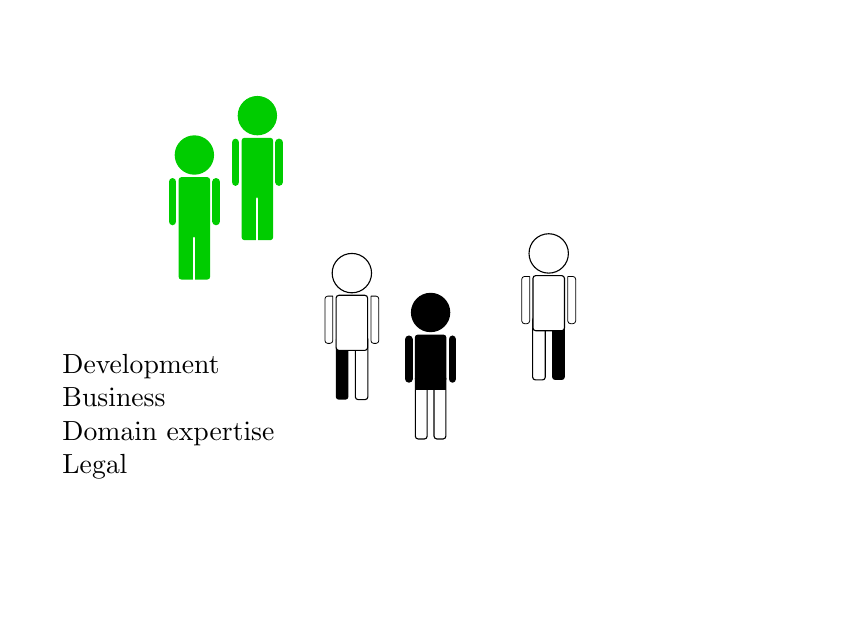
\begin{tikzpicture}
                \node[] at (0, 0) {};
                \node[] at (10, -7) {};

                \stickmantorso{(5, -3.5)}{black}
                \stickmanright{(4, -3)}{black}
                \stickmanleft{(6.5, -2.75)}{black}
                \node[align=left, anchor=west] at (0.2, -5) {
                    Development\\
                    Business\\
                    Domain expertise\\
                    Legal\\
                };

                \stickman{(2, -1.5)}{green!80!black}
                \stickman{(2.8, -1)}{green!80!black}
            \end{tikzpicture}
        }
        \only<2-4>{
            \begin{tikzpicture}
                \centering
                \node[] at (-0.25, 0.25) {};
                \node[] at (9.75, -6.25) {};

                \node[inner sep=0pt, draw=black, anchor=north west] at (0, 0) {
                    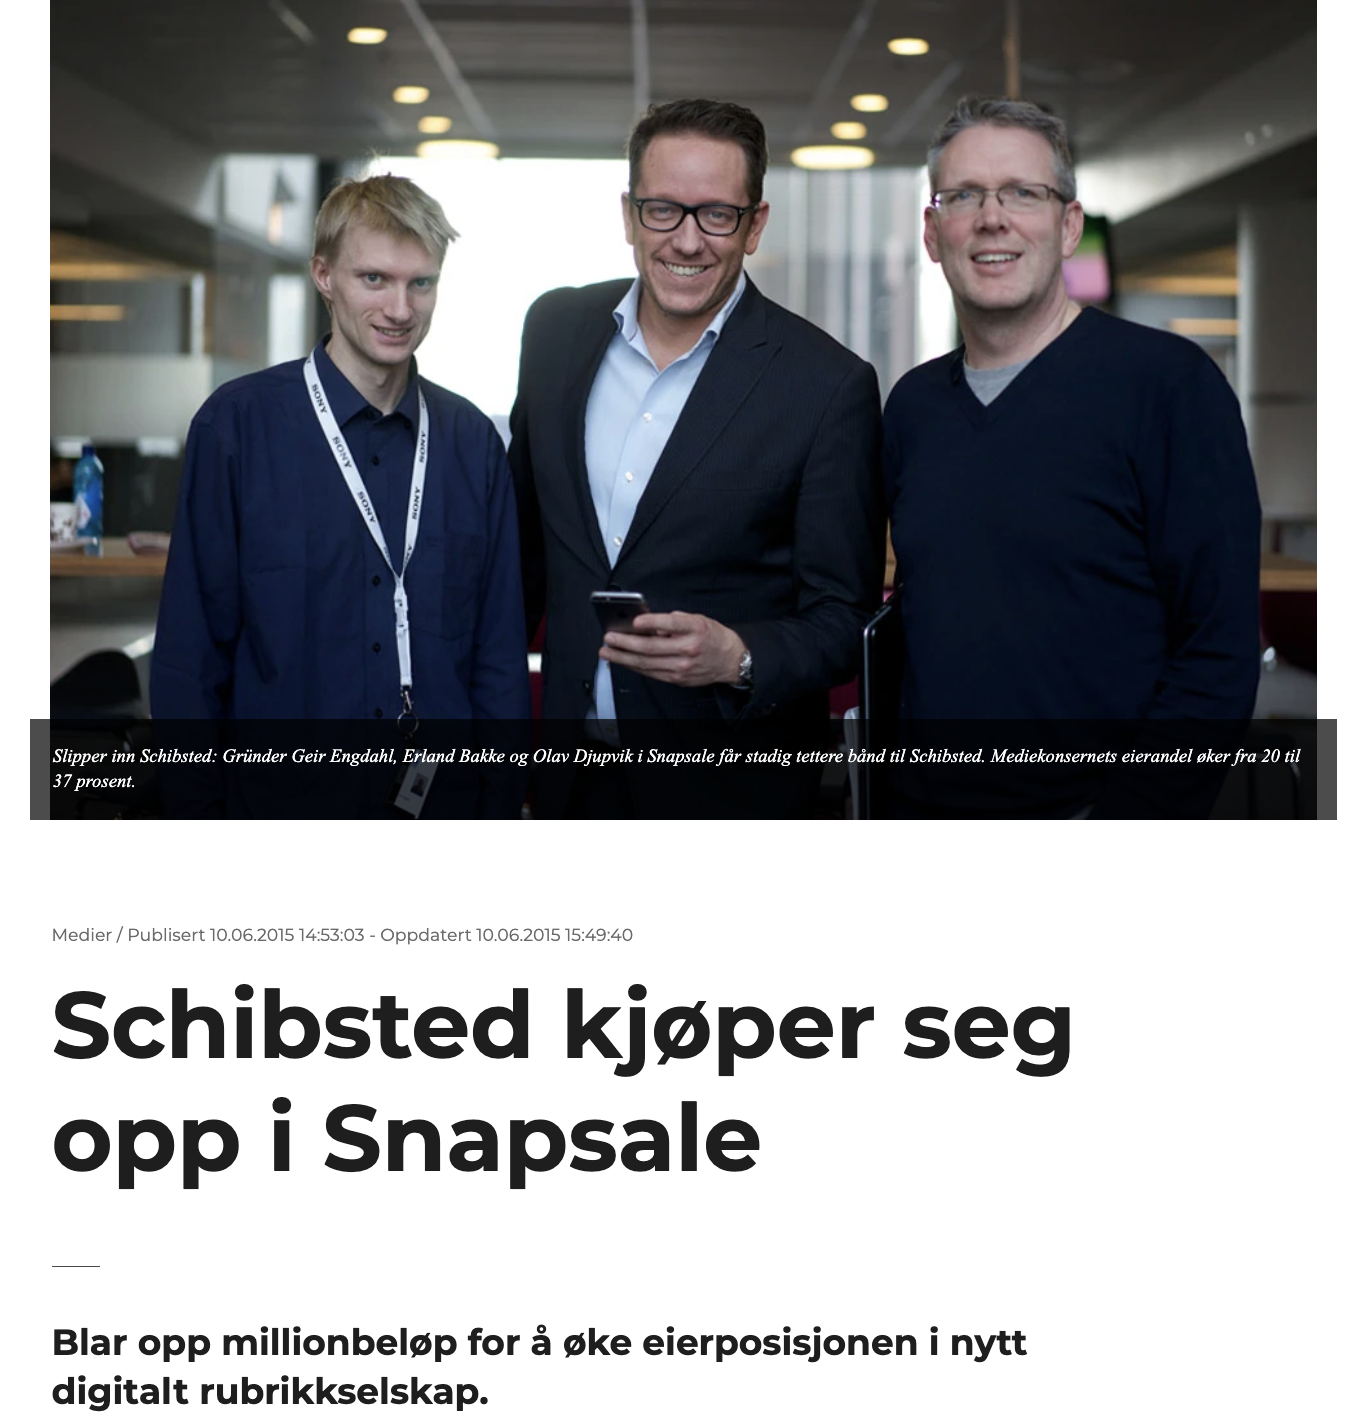
\includegraphics[height=5cm]{data/investering.png}
                };

                \only<3-4>{
                    \node[inner sep=0pt, draw=black, anchor=north west] at (2, -0.5) {
                        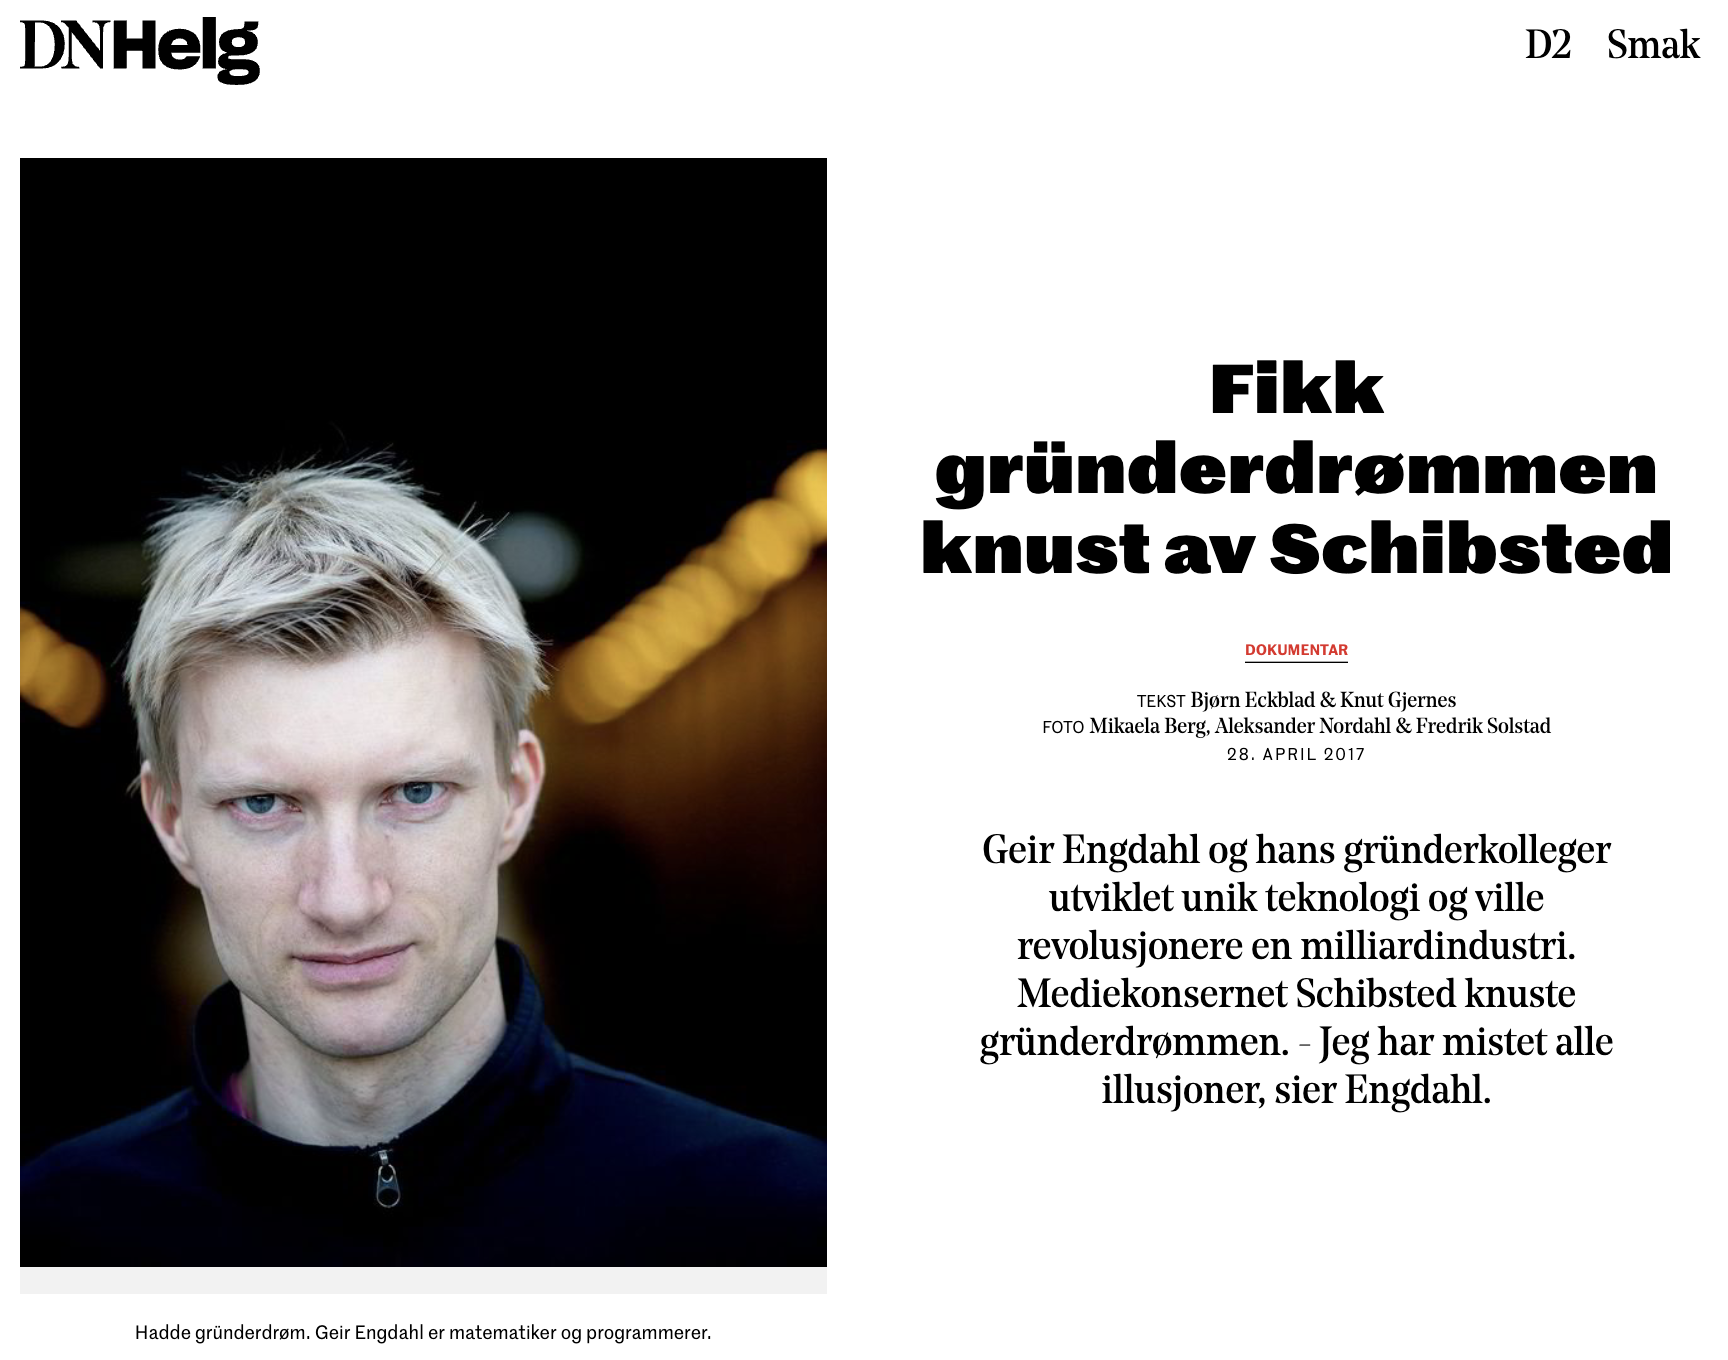
\includegraphics[height=5cm]{data/knust.png}
                    };
                }

                \only<4>{
                    \node[inner sep=0pt, draw=black, anchor=north west] at (4, -1) {
                        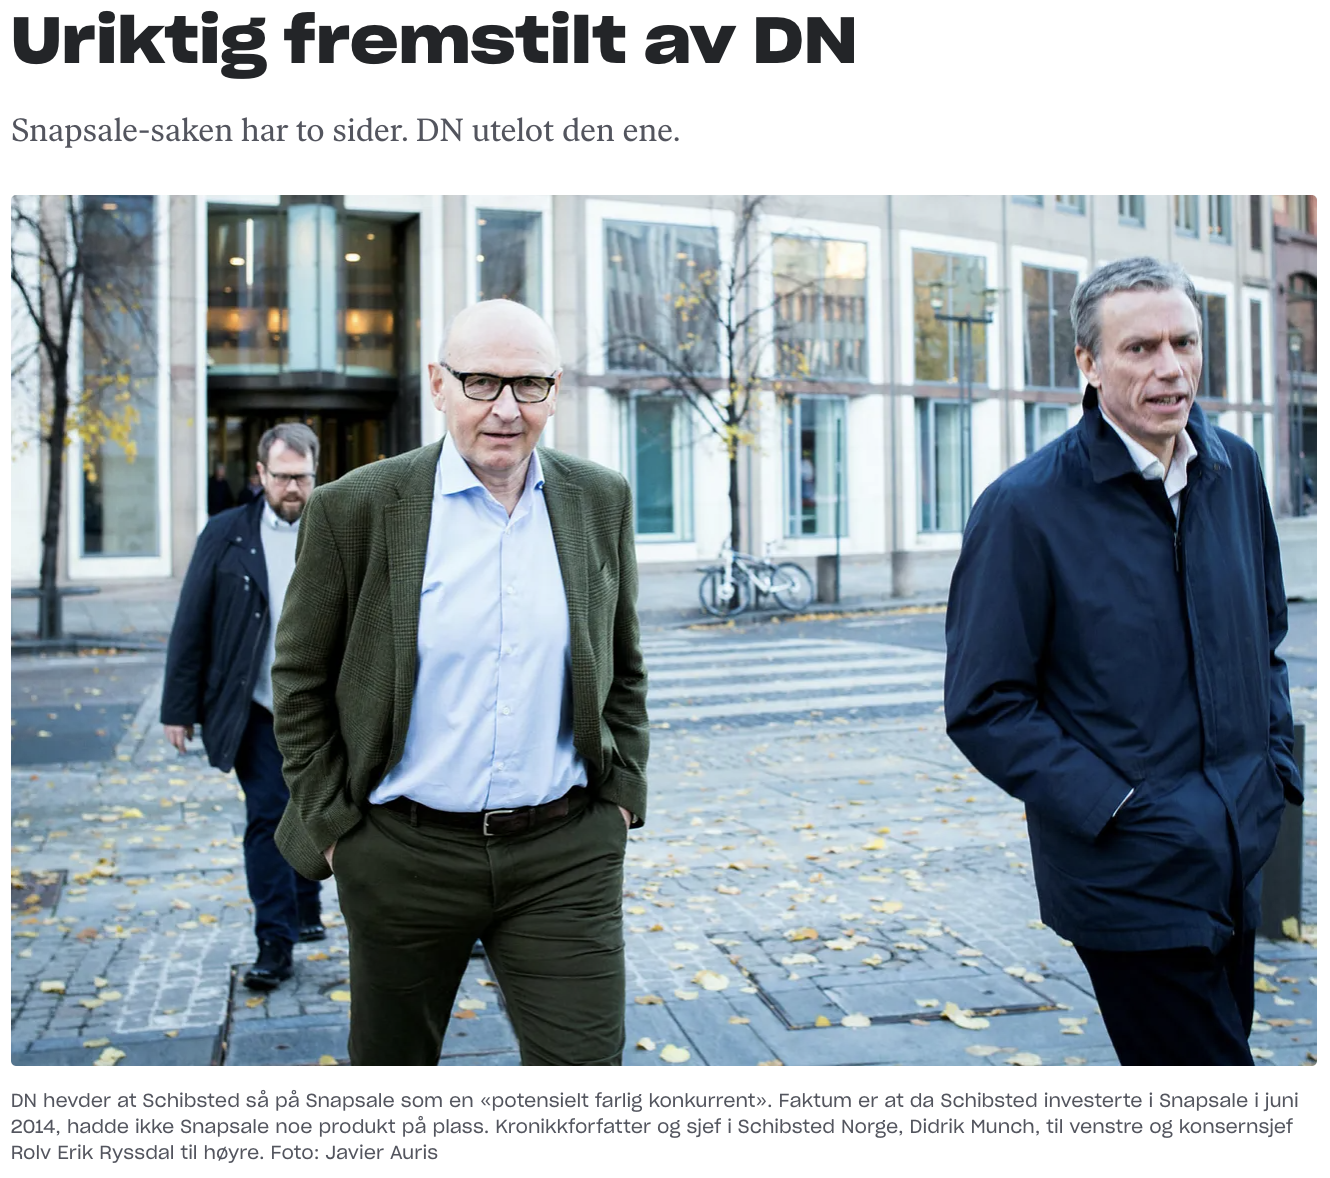
\includegraphics[height=5cm]{data/motsvar.png}
                    };
                }
            \end{tikzpicture}
        }
    \end{frame}

    \section{Resources}

    \begin{frame}{Resources: Inven2}
        \begin{tikzpicture}
            \node[] at (0, 0) {};
            \node[] at (10, -7) {};

            \node[anchor=north west] (inven2) at (0.4, -0.5) {
                
\includegraphics[width=2cm]{data/inven2.png}
            };
            \node[anchor=west] at (inven2.east) {
                Technology transfer organization for UiO/OUS
            };
            \only<2-3>{
                \node[] at (5, -3) {
                    
\includegraphics[width=7cm]{data/inven2_pitch.png}
                };
            }
            \only<3>{
                \node[] at (1.7, -5) {
                    
\includegraphics[width=3cm]{data/inven2_invention.png}
                };
                \node[] at (5, -5) {
                    
\includegraphics[width=3cm]{data/inven2_result.png}
                };
                \node[] at (8.3, -5) {
                    
\includegraphics[width=3cm]{data/inven2_guide.png}
                };
            }
        \end{tikzpicture}
    \end{frame}

    \begin{frame}{Resources: Growth house}
        \begin{tikzpicture}
            \node[] at (0, 0) {};
            \node[] at (10, -7) {};
            \only<1>{
                \node[anchor=north west] at (0, 0) {
                    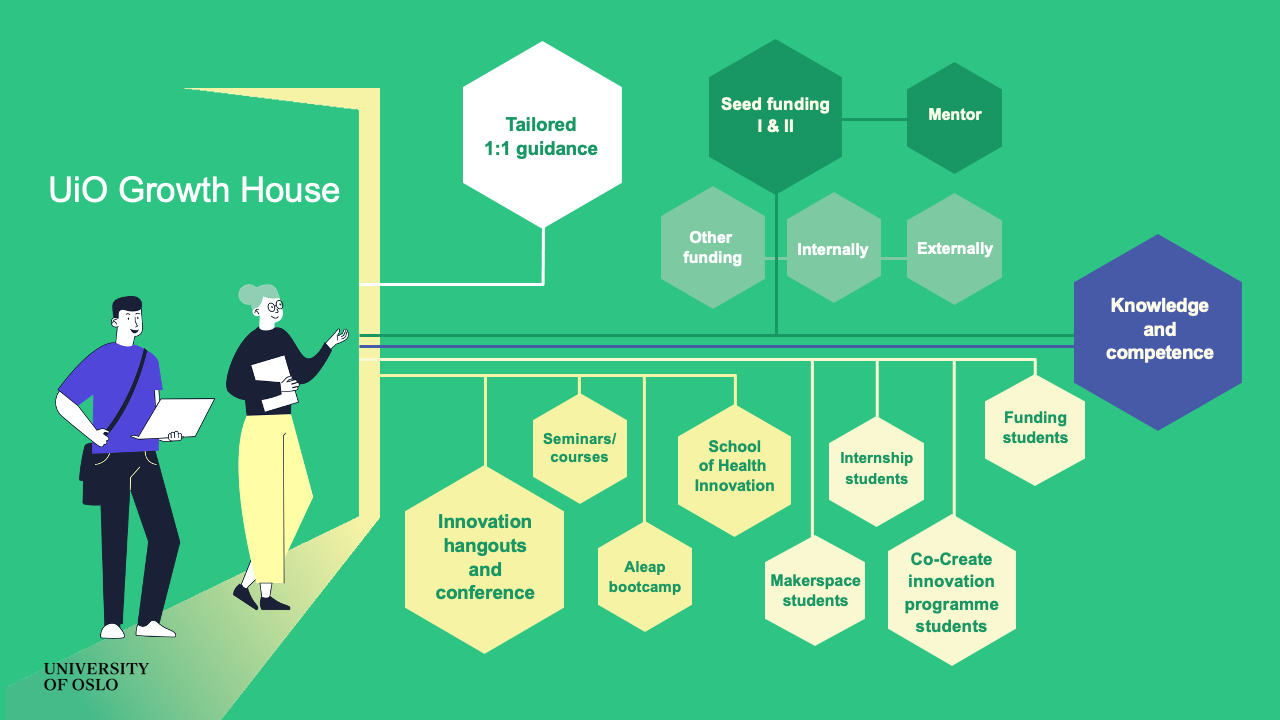
\includegraphics[
                        height=5.8cm,
                        trim={0 0 23.3cm 0},
                        clip=true
                    ]{data/growth_house_services.png}
                };
            }
            \only<2>{
                \node[anchor=north west] at (0, 0) {
                    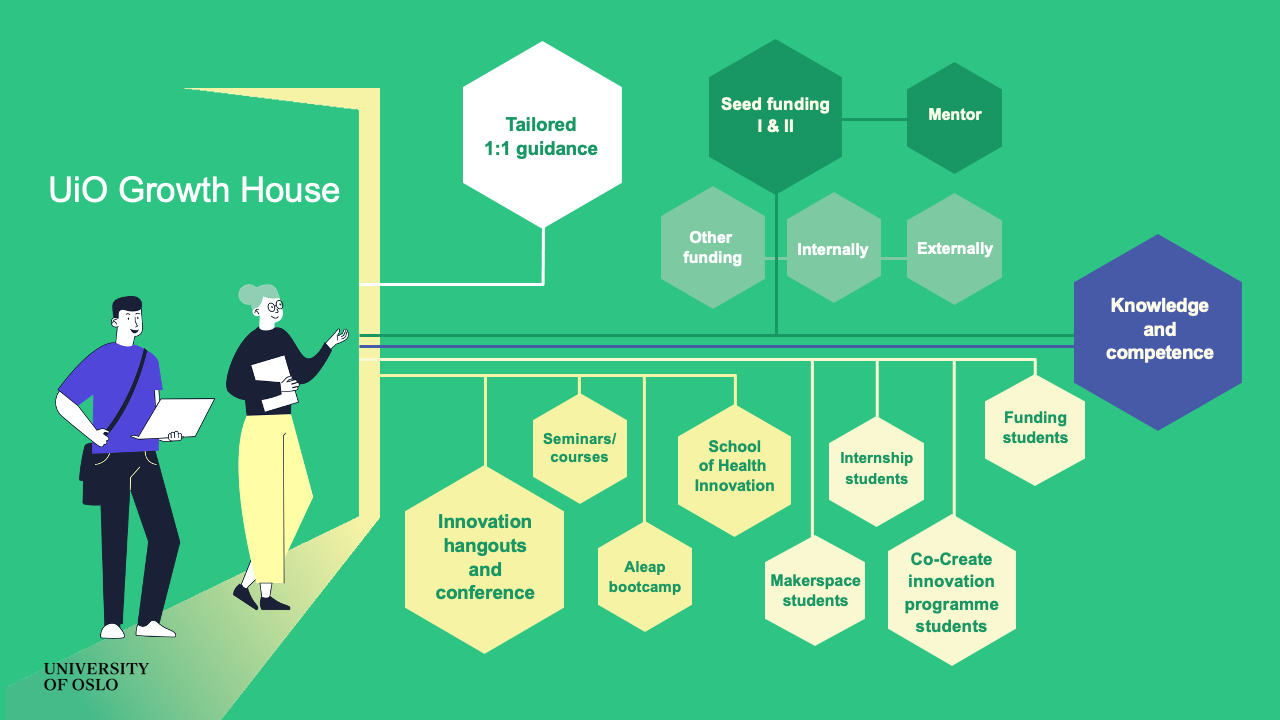
\includegraphics[height=5.8cm]{data/growth_house_services.png}
                };
            }
        \end{tikzpicture}
    \end{frame}

    \begin{frame}{Resources: Funding at UiO}
        \begin{tikzpicture}
            \node[] at (0, 0) {};
            \node[] at (10, -7) {};

            \node[anchor=north] at (5, 0) {
                
\includegraphics[width=6cm]{data/innovasjonsprisen.png}
            };

            \node[anchor=south] at (5, -7.5) {
                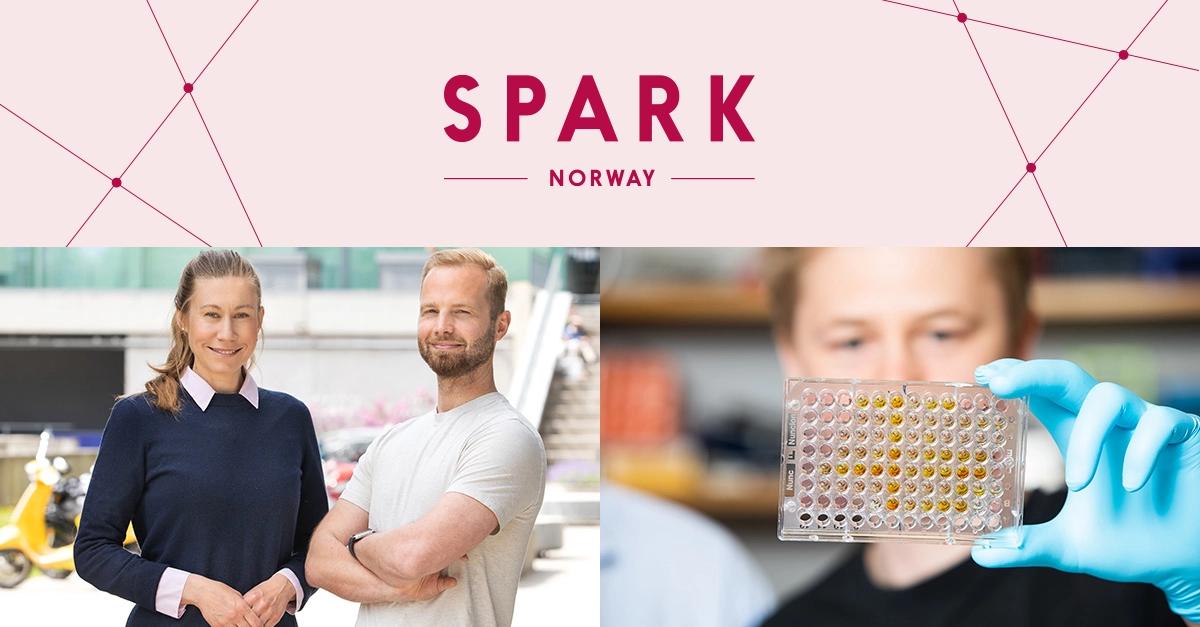
\includegraphics[width=8.5cm]{data/spark.png}
            };
        \end{tikzpicture}
    \end{frame}

    \begin{frame}{Resources: Funding outside UiO}
        \begin{tikzpicture}
            \node[] at (0, 0) {};
            \node[] at (10, -7) {};

            \node[anchor=south, inner sep=0pt, draw=black, fill=white] at (5, -6) {
                
\includegraphics[width=3cm]{data/innovasjon_norge.png}
            };
            \node[align=left] at (5.1, -2.5) {
                \begin{minipage}{8.3cm}
                    \begin{center}
                        \underline{\textbf{Grants and loans to start-ups}}
                    \end{center}
                    \begin{enumerate}
                        \item Start-up grant 1 (market validation): 200k NOK
                        \item Start-up grant 2 (concept development): 1M NOK
                        \item Start-up grant 3 (commercialization): 2M NOK
                        \item ???
                    \end{enumerate}
                \end{minipage}
            };
        \end{tikzpicture}
    \end{frame}

    \begin{frame}{Resources: Incubators}
        \centering
        \begin{tikzpicture}
            \node[draw=black, inner sep=0pt, fill=white] at (0, 0) {
                
\includegraphics[height=2.5cm]{data/startuplab.png}
            };
            \node[draw=black, inner sep=0pt, fill=white] at (6, 0) {
                
\includegraphics[height=2.5cm]{data/aleap.png}
            };
        \end{tikzpicture}
    \end{frame}

    \section{Thank you!}
\end{document}
